% Two-panel polarity diagnostic: existing nine FE solves at 48x24, classical clamp.
% Affine model V_E=0.0152918583*alpha1+0.0325316605*alpha3 (alpha in 1e-6 K^-1).
% Max absolute residual on the 9 solved points: 2.3e-14 V.
% All dashed segments outside the sampled parameter ranges are analytical
% extensions, NOT new FE runs. No joint alpha covariance is inferred.
\begin{figure}[t]
\centering
\begin{minipage}[t]{0.49\linewidth}
\centering
\begin{tikzpicture}
\begin{axis}[
 width=0.94\linewidth,height=6.3cm,
 xmin=9,xmax=34,ymin=-16,ymax=0,
 xlabel={$\alpha_1$ ($10^{-6}$ K$^{-1}$)},
 ylabel={$\alpha_3$ ($10^{-6}$ K$^{-1}$)},
 title={(a) Sampled pairs and polarity boundary},
 title style={font=\footnotesize},
 tick label style={font=\footnotesize},
 label style={font=\footnotesize},
 grid=major,
]
\addplot[only marks,mark=*,mark size=1.7pt,blue]
 table[x expr=\thisrow{alpha1}*1e6,
       y expr=\thisrow{alpha3}*1e6,col sep=comma]
 {program/verification/results/alpha_grid.csv};
\addplot[only marks,mark=square*,mark size=2.4pt,red]
 coordinates {(10.9,-6.45)};
\addplot[only marks,mark=star,mark size=3pt,black]
 coordinates {(21.8,-4.3)};
% Boundary segment inside original sampled parameter domain:
\addplot[red,thick,domain=10.9:13.72185,samples=2] {-0.4700607985298136*x};
\addplot[red,dashed,domain=13.72185:34,samples=2] {-0.4700607985298136*x};
\end{axis}
\end{tikzpicture}
\end{minipage}\hfill
\begin{minipage}[t]{0.49\linewidth}
\centering
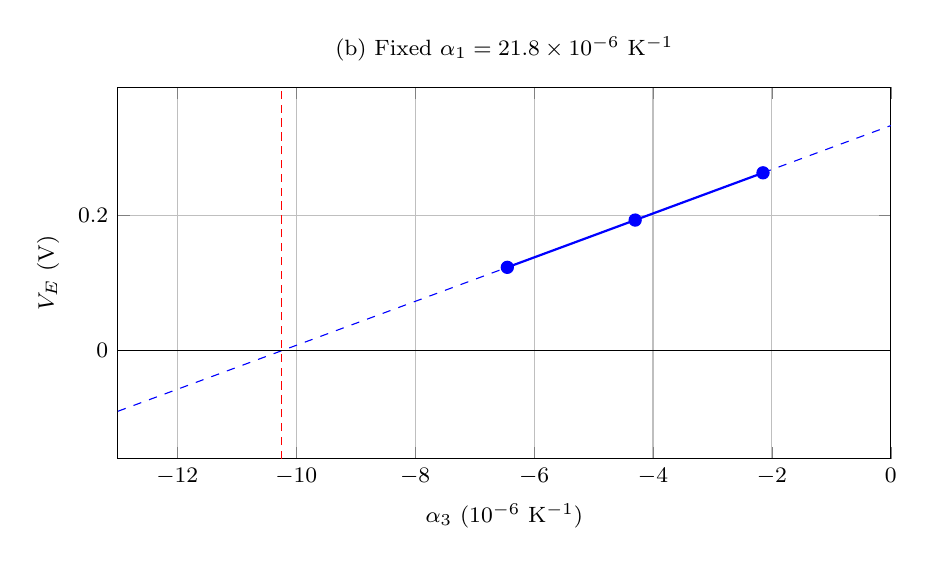
\begin{tikzpicture}
\begin{axis}[
 width=0.94\linewidth,height=6.3cm,
 xmin=-13,xmax=0,ymin=-0.16,ymax=0.39,
 xlabel={$\alpha_3$ ($10^{-6}$ K$^{-1}$)},
 ylabel={$V_E$ (V)},
 title={(b) Fixed $\alpha_1=21.8\times10^{-6}$ K$^{-1}$},
 title style={font=\footnotesize},
 tick label style={font=\footnotesize},
 label style={font=\footnotesize},
 grid=major,
]
\addplot[blue,dashed,domain=-13:-6.45,samples=2]
 {0.0152918583*21.8 + 0.0325316605*x};
\addplot[blue,thick,domain=-6.45:-2.15,samples=2]
 {0.0152918583*21.8 + 0.0325316605*x};
\addplot[blue,dashed,domain=-2.15:0,samples=2]
 {0.0152918583*21.8 + 0.0325316605*x};
\addplot[only marks,mark=*,mark size=2.2pt,blue]
 coordinates {(-6.45,0.12353330079707622) (-4.3,0.19347637076881116) (-2.15,0.2634194407405431)};
\addplot[red,densely dashed]
 coordinates {(-10.24732540795,-0.16) (-10.24732540795,0.39)};
\addplot[black,thin] coordinates {(-13,0) (0,0)};
\end{axis}
\end{tikzpicture}
\end{minipage}
\caption{Polarity of the piezoelectric--thermal response on the $48\times24$
 classical-clamp mesh. (a) The nine simulated thermal-expansion pairs and
 the $V_E=0$ boundary implied by their affine dependence; the dashed
 continuation lies outside the sampled parameter domain. (b) The three
 computed $V_E$ values at the nominal $\alpha_1$, together with the affine
 response and its predicted zero at $\alpha_3\approx-10.25\times10^{-6}$~K$^{-1}$.
 Blue circles mark computed pairs, the red square marks the negative-voltage
 case, and the black star marks the nominal pair. Solid lines indicate
 the sampled parameter range; dashed lines extend the fixed-mesh affine model
 without additional finite-element runs.}
\label{fig:alpha-polarity}
\end{figure}
